\documentclass{book}


\usepackage[spanish]{babel}
\usepackage[utf8]{inputenc}
\usepackage[T1]{fontenc}
\usepackage{graphicx}

\title{grecks}
\date{\today}
\author{Alexia Rodríguez Miranda\thanks{geniuswolfgang}}

\begin{document}
\maketitle

\chapter{Alexia}

\section{un poco sobre mi}
\textbf{ADVERTENCIA. Lees esto a conciencia de que son tonterias.}

Me llaman Alexia, realmento solo aspiro a la felicidad, ya lo se, super cliche pero pues...me gusta, voy en la facultad de ciencias, porque, no es que sea especialmente buena, de hecho no lo soy, pero vale la pena seguir, es divertido :) ahhh y vengo de prepa 9, tome alguna clase de programacion c++ y pues me gusto, así que aquí estoy. 


Me gusta mucho leer los libros~\cite{torres,comunidad,retorno}

\subsection{hobbies}

\begin{enumerate}
\item cantar
\item respirar (hacer yoga y ballet)
\item tocar el piano
\end{enumerate}

\begin{figure}[h]
  \centering
  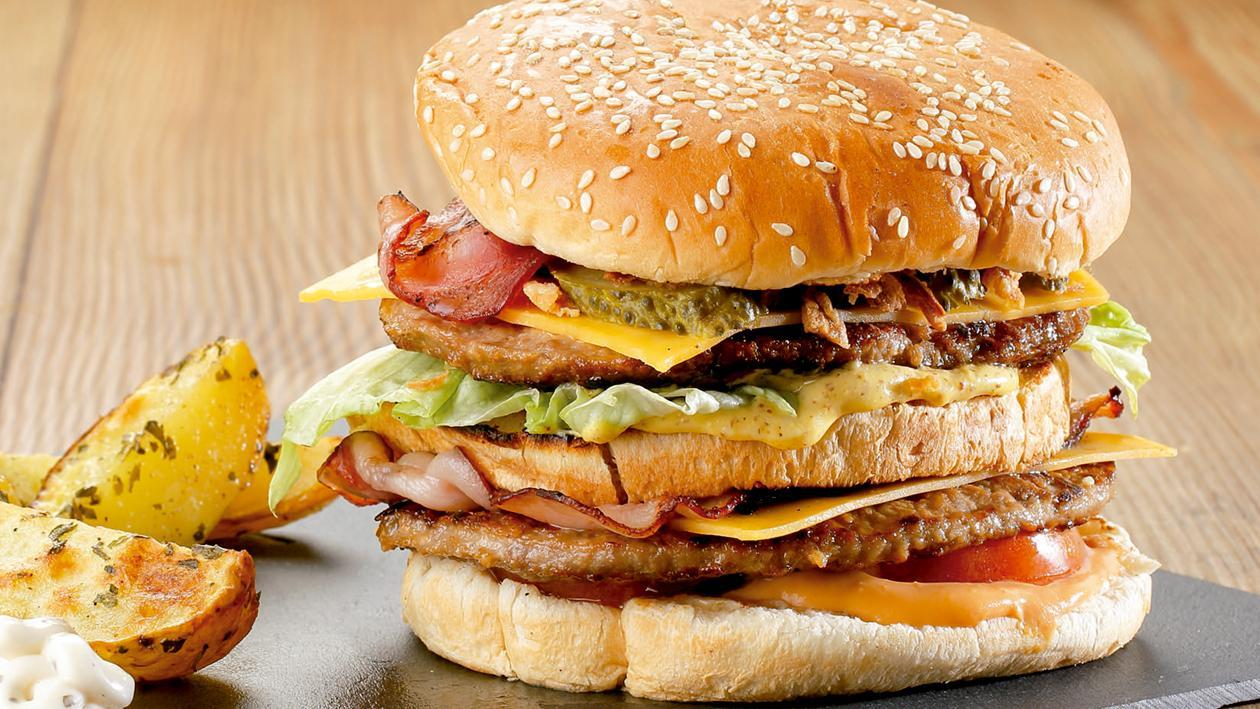
\includegraphics[scale=0.10]{IMG/6.jpg}
  \caption{my love}
  \label{fig:hamburguesa}
\end {figure}

Podemos ver una deliciosa hambueguesa llamada comunmente por mi: amor
\textbf{figura}~\ref{fig:hamburguesa}.

\begin{itemize}
\item $c^{-ba}$
\item $x=-b_a \pm \frac{5}{\sqrt{9}}$
 \end{itemize}

\begin{tabular}{|l | c | r|}
  \hline
  comida & yet & porcino \\
  \hline
  pepinillos & gorra & carpa \\
  \hline
  
\end{tabular}

\end{document}


